\documentclass[11pt,a4paper]{article}
\usepackage[T1]{fontenc}
\usepackage{lmodern}
\usepackage[margin=24mm,headheight=15pt]{geometry}
\usepackage{amsmath,amssymb,amsthm}
\usepackage{booktabs,longtable,tabularx,array}
\usepackage{graphicx,xcolor,microtype,enumitem}
\usepackage{fancyhdr}
\usepackage[unicode,colorlinks=true,linkcolor=blue!45!black,urlcolor=blue!45!black,citecolor=blue!45!black]{hyperref}
\hypersetup{pdftitle={Independent verification: similariton noise and normal-dispersion squeezing},pdfauthor={ChatGPT, GPT-6 Astra Pro},pdfsubject={Independent derivations, numerical reproduction, counterexamples, and literature assessment}}
\pagestyle{fancy}
\fancyhf{}
\fancyhead[L]{\small Independent verification of nonlinear-fiber claims}
\fancyhead[R]{\small 18 October 2026}
\fancyfoot[C]{\thepage}
\setlength{\parindent}{0pt}
\setlength{\parskip}{6pt}
\setlist{nosep,leftmargin=1.6em}
\renewcommand{\arraystretch}{1.18}
\newcolumntype{Y}{>{\raggedright\arraybackslash}X}
\newcommand{\dd}{\mathrm d}
\newcommand{\Var}{\operatorname{Var}}
\newcommand{\Cov}{\operatorname{Cov}}
\newcommand{\Tr}{\operatorname{Tr}}
\newcommand{\sinc}{\operatorname{sinc}}
\newcommand{\R}{\mathbb R}
\newcommand{\Nph}{N_{\mathrm{ph}}}
\newcommand{\eps}{\varepsilon}
\newcommand{\lzero}{\lambda_0}
\newcommand{\doi}[1]{\href{https://doi.org/#1}{doi:#1}}
\newtheorem{proposition}{Proposition}
\newtheorem{lemma}{Lemma}
\newtheorem{definition}{Definition}
\graphicspath{{../weak/}{../similariton/}{../strong/}}
\begin{document}
\hypersetup{pageanchor=false}
\begin{titlepage}
\vspace*{12mm}
{\color{blue!45!black}\large INDEPENDENT TECHNICAL VERIFICATION\par}
\vspace{8mm}
{\LARGE\bfseries Quantum noise around amplifier similaritons\par}
\vspace{3mm}
{\LARGE\bfseries and squeezing in normal-dispersion fibers\par}
\vspace{10mm}
{\large Derivations, independent propagation, counterexamples, and assessment of novelty\par}
\vspace{10mm}
\begin{tabularx}{\textwidth}{@{}lY@{}}
Repository & \url{https://github.com/nrivera494/analytical-nl-discovery} \\
Snapshot & \small\path{970bfe756b131094872de351ff91ab46a537d9b2} \\
Primary targets & C-20261008-claude-a-02; C-20261010-claude-a-01, item 5; C-20261010-claude-b-01 \\
Prepared & 18 October 2026, by ChatGPT (GPT-6 Astra Pro) with independent parallel derivation and implementation tasks \\
Companion & Reproducibility archive: original verification code, raw results, detailed derivation notes, and this report's source \\
\end{tabularx}
\vspace{10mm}
\textbf{Main conclusion.} Both priority asymptotics survive independent verification in a precisely delimited linearized model. The similariton powers are \emph{variance} envelopes of photon-normalized shape variables. The weak-dispersion formula describes the best arbitrary-mode quadrature variance, which bounds filtered photon-counting noise. Several stronger interpretations do not survive: complete amplifier noise does not forbid all squeezing, one collective phase power is incorrect, and smooth hydrodynamics cannot simply be continued through wave breaking.

\textbf{Level of proof.} This report proves the reduced similariton mode spectrum, the effective oscillator minimum, a bandwidth counterexample, and a finite-dimensional symplectic asymptotic. It derives the weak optical law directly from the full linearized generator and reproduces it numerically. A global continuum spectral-localization theorem and a postbreaking tangent-map limit remain unproved; they are explicitly separated from the demonstrated results.
\vfill
\small This is a computational and analytical verification, not an experimental validation. Numerical precision reported below refers to stated discretizations and convergence tests. It does not bound error from omitted Raman response, gain saturation, higher dispersion, loss, or finite material bandwidth.
\end{titlepage}
\hypersetup{pageanchor=true}
\pagenumbering{roman}
\begingroup
\setlength{\parskip}{0pt}
\small
\tableofcontents
\endgroup
\clearpage
\pagenumbering{arabic}

\section{Conclusions and evidence standard}

The repository's preliminary pass labels were not used as evidence. The three target claim cards, their derivation notes and numerical scripts, related scope claims, and later review notes were inspected at a pinned snapshot. No repository solver was imported into the new calculations. The verification uses a finite-volume spatial operator and differential covariance propagation for the reduced amplifier problem, an exact lens-coordinate NLSE and adjoint for its full-field checks, an eighth-order finite-difference/DOP853 solver for weak dispersion, and a separate fourth-order Fourier symplectic tangent solver for the normal-dispersion crosschecks.

\begin{longtable}{@{}p{.27\textwidth}p{.23\textwidth}p{.44\textwidth}@{}}
\toprule
Claim or interpretation & Verdict & Strongest statement supported here \\
\midrule\endhead
Similariton shape powers $G^{1/3}$ and $G^{5/3}$ & Verified in leading hydrodynamics; independently reproduced & Fixed low-order modes have these photon-normalized \emph{variance envelopes}; rms powers are $G^{1/6}$ and $G^{5/6}$. Full NLSE checks support the lowest shape mode. \\
Spectral covariance ratio $G^{-2/3}$ & Verified for the stated finite core projection & The first five spectral Legendre components become dominated by an energy mode. Oscillating prefactors and the chosen covariance metric matter. This is not a theorem for the entire quantum field. \\
Phase--energy deficit $G^{-2/3}$ & Verified in the reduced model & The matched-mean phase contains a quadrupole shape residual beneath a larger energy-driven phase. Generic nondegenerate covariance gives the stated envelope. \\
Matched-LO $C_{PP}\propto G/\eps_0^2$ & Incorrect as a gain asymptotic & At fixed $\Gamma,\eps_0$, $C_{PP}\sim(32n_{sp}/9)G\Phi_{NL}^{2}\propto G^{7/3}/\eps_0^2$. \\
ASE implies no squeezing & Incorrect as an unconditional statement & A complete-noise short-amplifier counterexample gives $\lambda_{LO}=0.8964865<1$. This does not establish large-gain similariton squeezing. \\
Gaussian weak-dispersion square root & Independently derived and reproduced & At fixed $\Phi>0$, the coefficient is $\sqrt{2/3}\,\Phi/\sqrt{1+\Phi^2}$ and rms width is $T_0(y/24)^{1/4}$. A global continuum lower-bound theorem still needs spectral localization. \\
Peak order $2m$ changes exponent & Verified effective reduction and numerical tests & Excess power $m/(m+1)$ and width power $1/(2m+2)$; quadratic, quartic, and sextic peaks tested independently. \\
Empirical next coefficient $c_2\simeq1$ & Refined & A full local second-order calculation supplies a closed $c_2(\Phi)$, approaching $2\sqrt6/5$ at large $\Phi$. This remains a formal local expansion with numerical support. \\
Unrestricted $\lambda_{\min}$ equals optimum passive-filter Fano factor & Not established; generally different optimizations & $\lambda_{\min}$ bounds passive-filter counting noise. A shaped LO attains it when an $L^2$ minimizing mode exists; otherwise an LO sequence approaches it. \\
Strong-dispersion $\Lambda(Z)/N^2$ & Conditional theorem plus reliable evidence & Proven for bounded symplectic blocks with a regular limit; independently reproduced before breaking and at one tested postbreaking distance. \\
Same classical hydrodynamic map beyond breaking & Unproved and insufficiently defined & Beyond gradient catastrophe, define any limit from full NLSE tangent maps or a justified oscillatory modulation theory. The smooth Euler map has ceased to exist. \\
\bottomrule
\end{longtable}

\paragraph{What is not claimed.} This investigation does not prove a uniform sharp-edge quantum error estimate, universal attraction of arbitrary input pulses, an unrestricted infinite-mode covariance rank-one theorem, a globally rigorous weak-dispersion covariance theorem, or an all-distance postbreaking squeezing theorem. The Raman and polarization branches of C-20261010-claude-a-01 are outside the requested priority result and have not been independently certified here. These boundaries are material to the interpretation, not reasons to discard the reproduced leading laws.

\section{Common model, quantum normalization, and observables}

Let $A(z,t)$ be a classical mean envelope in $\mathrm W^{1/2}$, so $P=|A|^2$ is power and $\Nph=\int P\,\dd t/(\hbar\omega_0)$ is coherent-signal photon number, equal to the total mean at leading bright-field order. Normal dispersion means $\beta_2>0$ in
\begin{equation}\label{eq:mean}
\partial_z A=-\frac{i\beta_2}{2}\partial_t^2 A+i\gamma |A|^2A+\frac g2 A.
\end{equation}
Here $g$ is the \emph{power/energy} gain coefficient: $G=e^{gz}$ and field gain is $\sqrt G$. For the passive squeezing problem $g=0$. Instantaneous Kerr response, one polarization and spatial mode, unsaturated frequency-flat gain when present, and no loss or Raman reservoir are assumptions of the calculation, not general properties of a physical fiber.

Write the photon-flux operator as $\hat a=A/\sqrt{\hbar\omega_0}+\hat b$, with $[\hat b(t),\hat b^\dagger(t')]=\delta(t-t')$. The exact first variation of \eqref{eq:mean} is the Bogoliubov equation
\begin{equation}\label{eq:bdg}
\dd\hat b=\left[-\frac{i\beta_2}{2}\partial_t^2\hat b
+i\gamma(2|A|^2\hat b+A^2\hat b^\dagger)+\frac g2\hat b\right]\dd z+\dd\hat F.
\end{equation}
Define $X=\hat b+\hat b^\dagger$ and $P_q=(\hat b-\hat b^\dagger)/i$. Then $[X(t),P_q(t')]=2i\delta(t-t')$, and vacuum has symmetrized covariance $I$. A normalized complex local oscillator $h$, $\int|h|^2\dd t=1$, measures $Q_h=\int(h^*\hat b+h\hat b^\dagger)\dd t$, with vacuum variance one.

For coherent input and a complete lossless discretization, the real tangent map $M$ is symplectic and the output covariance is:
\begin{equation}\label{eq:sympl}
MJM^{\mathsf T}=J,\qquad V=MM^{\mathsf T},\qquad VJV=J.
\end{equation}
The \emph{ordinary} eigenvalues of $V$ occur in reciprocal pairs, and
\begin{equation}\label{eq:recip}
\lambda_{\min}(V)=\|M\|_2^{-2}.
\end{equation}
They are not the symplectic eigenvalues used in Williamson's theorem; those are all one for this pure Gaussian covariance. A covariance minimum below one is quadrature squeezing. A reduction relative to a noisier amplified baseline is not sufficient.

\subsection{The amplifier reservoir cannot be omitted}

With the repository's $n_{sp}\ge1$ convention, the independent-increment reservoir has
\begin{align}
\langle\dd\hat F^\dagger(t)\dd\hat F(t')\rangle&=gn_{sp}\delta(t-t')\dd z,\\
\langle\dd\hat F(t)\dd\hat F^\dagger(t')\rangle&=g(n_{sp}-1)\delta(t-t')\dd z,\\
[\dd\hat F(t),\dd\hat F^\dagger(t')]&=-g\delta(t-t')\dd z.
\end{align}
The negative reservoir commutator cancels the commutator growth from the gain drift. In physical quadratures the covariance channel is
\begin{equation}\label{eq:ase}
V(z)=M(z,0)V(0)M(z,0)^{\mathsf T}
+\int_0^z M(z,s)g(2n_{sp}-1)I M(z,s)^{\mathsf T}\dd s.
\end{equation}
For a linear amplifier this gives
\begin{equation}\label{eq:linearamp}
V_{\mathrm{lin}}=[G+(2n_{sp}-1)(G-1)]I.
\end{equation}
Replacing $V$ by $MM^{\mathsf T}$ with a gain-containing $M$ misses amplifier-added noise and violates the canonical commutator. These quantum restrictions are established amplifier physics \cite{caves,drummondcorney}; the audit explicitly includes both input-vacuum and both reservoir quadratures where a full quantum covariance is reported.

\subsection{Filtered Fano factors and optimum homodyne modes}

For a bright output, linearized photon counting projects fluctuations along the transmitted coherent amplitude. Its normalized variance is a covariance Rayleigh quotient for that particular detection vector. A passive spectral filter restricts that vector and, if partially transmitting, mixes in vacuum. Optimizing a normalized complex LO allows all real quadrature directions, giving $\lambda_{\min}(V)$. Thus, when $\lambda_{\min}\le1$,
\begin{equation}\label{eq:filterbound}
F_{\text{passive filter}}\ \ge\ \lambda_{\min}(V),
\end{equation}
with equality requiring a separate readout construction. This distinction is already explicit in Opatrn\'y, Korolkova and Leuchs, Eqs.\ (52)--(64) \cite{opatrny}. The weak-dispersion claim card defines the covariance quantity correctly; describing the result as the attained optimum \emph{filtered Fano factor} would overstate what has been calculated.

\section{Problem 1: amplifier-similariton shape exponents}

\subsection{Background and exact leading fluctuation separation}

Set
\begin{equation}
L_D=\frac{T_0^2}{\beta_2},\quad L_{NL}=\frac1{\gamma P_0},\quad
\eps_0=\sqrt{\frac{L_{NL}}{L_D}},\quad
\zeta=\frac z{\sqrt{L_DL_{NL}}},\quad \Gamma=g\sqrt{L_DL_{NL}},\quad
\tau=\Gamma\zeta=\ln G.
\end{equation}
In the dispersionless hydrodynamic approximation the parabolic mean has
\begin{equation}\label{eq:parabola}
P=P_0\frac G{a}(1-\xi^2),\qquad \xi=\frac{t}{T_0a},\quad |\xi|<1,
\qquad a_{\zeta\zeta}=\frac{2G}{a^2}.
\end{equation}
The associated fluid velocity $v=-\beta_2\partial_t\arg A$ is $(a_z/a)t$. The asymptotic solution is
\begin{equation}\label{eq:asymwidth}
a\sim A_GG^{1/3},\qquad A_G=(18/\Gamma^2)^{1/3},\qquad P_{pk}\propto G^{2/3},\qquad \Nph=N_0G.
\end{equation}
This background scaling is established similariton physics \cite{fermann,kruglov}. The parabolic profile is a leading interior approximation: a sharp compact-support square-root envelope does not remove the dispersive edge layer.

Attraction within the positive-width ODE can also be shown independently. Put $b=a/(A_Ge^{\tau/3})$. Then
\begin{equation}
b_{\tau\tau}+\frac23b_\tau+\frac b9=\frac1{9b^2},\qquad
\mathcal E=\frac12b_\tau^2+\frac{b^2}{18}+\frac1{9b},\qquad
\mathcal E_\tau=-\frac23b_\tau^2.
\end{equation}
Positive-width sublevel sets are compact and bounded away from zero, and the only invariant zero-dissipation set is $b=1,b_\tau=0$. Thus the width tends to the self-similar member. This proves attraction inside the parabolic hydrodynamic family, not for arbitrary full-NLSE initial data.

Define the \emph{peak-normalized absolute density} perturbation and physical phase perturbation by
\begin{equation}
\delta P=P_{pk}n(\xi),\qquad \delta\arg A=p(\xi).
\end{equation}
In particular, $n$ is not the local relative perturbation $\delta P/P=n/(1-\xi^2)$. Linearizing the continuity and phase equations, with advection removed by $\xi$, gives
\begin{equation}\label{eq:simlin}
n_\zeta=\frac{\eps_0}{a^2}\partial_\xi[(1-\xi^2)p_\xi],\qquad
p_\zeta=\frac{G}{\eps_0a}n.
\end{equation}
The spatial Sturm--Liouville operator has bounded regular eigenfunctions $P_l(\xi)$:
\begin{equation}
-\partial_\xi[(1-\xi^2)\partial_\xi P_l]=l(l+1)P_l,\qquad
\int_{-1}^1P_lP_m\dd\xi=\frac{2\delta_{lm}}{2l+1}.
\end{equation}
Writing $n=\sum n_lP_l$, $p=\sum p_lP_l$ therefore yields the independent leading blocks
\begin{equation}\label{eq:blocks}
n_{l,\zeta}=-\frac{\eps_0l(l+1)}{a^2}p_l,
\qquad p_{l,\zeta}=\frac{G}{\eps_0a}n_l.
\end{equation}
The separation is exact for the hydrodynamic parabolic background, including its width transient. It is not exact for the full NLSE with quantum pressure or a nonparabolic seed.

For $l\ge1$, eliminating $p_l$ and inserting \eqref{eq:asymwidth} gives
\begin{equation}\label{eq:simode}
n_{l,\tau\tau}+\frac23 n_{l,\tau}+\frac{l(l+1)}{18}n_l=0.
\end{equation}
For $l\ge2$,
\begin{equation}\label{eq:simmodes}
\begin{aligned}
n_l&=G^{-1/3}\{a_l\cos(\omega_l\ln G)+b_l\sin(\omega_l\ln G)\},\\
\omega_l&=\frac13\sqrt{\frac{l(l+1)}2-1},\qquad p_l=G^{1/3}\times\text{bounded oscillation}.
\end{aligned}
\end{equation}
These equations independently establish the reported real decay rate and frequency. For $l=0$, the first-order equation says $n_0$ is constant in homogeneous propagation; one must not infer an additional density solution by extending the eliminated equation to $l=0$. For $l=1$, $n_1=G^{-1/3}(a_1+b_1\ln G)$ is a repeated-root solution associated with centroid degrees of freedom.

\subsection{What the reported powers actually measure}

Photon-normalized shape variables are proportional to $\sqrt{\Nph}\,n_l$ and $\sqrt{\Nph}\,p_l$. Their actual modal vacuum metric is not automatically the identity, so these are not yet unit-vacuum canonical single-mode quadratures. Multiplying the variances from \eqref{eq:simmodes} by $\Nph=N_0G$ gives
\begin{equation}\label{eq:simpowers}
\boxed{\Var(\sqrt{\Nph}\,n_l)\ \text{has envelope }G^{1/3},\qquad
\Var(\sqrt{\Nph}\,p_l)\ \text{has envelope }G^{5/3}.}
\end{equation}
The rms powers are $G^{1/6}$ and $G^{5/6}$. The dimensionless density coefficient itself decays as $G^{-1/3}$, whereas its absolute physical power perturbation $P_{pk}n_l$ grows as $G^{1/3}$. These distinct normalizations happen to reuse one exponent and should not be conflated.

With distributed ASE, the leading density diffusion in these unnormalized comoving variables is proportional to $G^{-1}(1-\xi^2)\delta(\xi-\xi')\dd\tau$. A shape-mode covariance therefore contains, schematically,
\begin{equation}
G^{-2/3}\int_0^\tau e^{2s/3}e^{-s}B_l(s)\dd s,
\end{equation}
where $B_l$ is bounded and oscillatory. The integral converges, so continuous noise injection changes the leading prefactor, not the density variance power. The phase obtained from \eqref{eq:blocks} has the corresponding $G^{2/3}$ unnormalized variance. At any fixed regulated mode cutoff the phase-source contribution can also be propagated; it does not license dropping that source when certifying a quantum state.

For a nondegenerate stochastic covariance the surviving statement is a power envelope, often expressed as $\Theta(G^q)$ after excluding accidental null directions. A single deterministic mode can cross zero, so a pointwise lower bound on every realization is false. Logarithmic-gain oscillations also mean $G^{-q}\Var$ need not converge to a constant. Straight-line fits over short gain intervals are not a replacement for \eqref{eq:simode}.

\subsection{Commutators, edge noise, and what a block determinant proves}

Using $\rho_{pk}^{(\mathrm{phot})}T_0a=3\Nph/4$, the linearized equal-distance density--phase commutator is
\begin{equation}\label{eq:simcomm}
[n(\xi),p(\xi')]=\frac{4i}{3\Nph}\delta(\xi-\xi'),\qquad
[n_l,p_m]=\frac{2i(2l+1)}{3\Nph}\delta_{lm}.
\end{equation}
It changes with gain because the variables are normalized by a changing mean. The homogeneous $(p_l,n_l/\eps_0)$ drift has zero trace and determinant-one transfer matrices, but this does not by itself verify \eqref{eq:simcomm} for the physical gain channel. The reservoir in \eqref{eq:ase} is essential.

Even at the coherent input, phase noise in the formal sharp parabola has covariance proportional to
\begin{equation}\label{eq:edge}
\langle p(\xi)p(\xi')\rangle_{\mathrm{sym}}
=\frac{\delta(\xi-\xi')}{3\Nph(1-\xi^2)},\qquad
\int_{-1}^1\frac{P_l(\xi)P_m(\xi)}{1-\xi^2}\dd\xi.
\end{equation}
The projected integral is logarithmically divergent. Raw polynomial phase projections are not legitimate finite-variance quantum observables for the exactly sharp seed. Smooth physical field quadratures and a matched LO can remain well defined, but their evaluation requires the edge cancellations or a regularized full-field calculation. A covariance which keeps only density vacuum and density ASE is a leading classical covariance calculation, not a complete single-block quantum state. The card acknowledges that omission, but it does not prove its claimed uniform edge remainder.

\subsection{Independent numerical reproduction}

The finite-volume calculation discretizes the spatial operator on midpoint cells with zero boundary flux, diagonalizes that operator numerically, and integrates a differential Lyapunov equation for the covariance. The readouts use its own orthonormal numerical eigenfunctions, which converge to normalized Legendre polynomials; analytic Legendre values set signs only. This differs from directly inserting the repository's analytic block matrices and evaluating their quadratures. The density covariance retains its nondiagonal projected metric, including cross-mode noise.

For eight retained numerical modes, 32--1024 midpoint cells, $\Gamma=\sqrt{18}$ and $n_{sp}=1$, the independently computed density-mode eigenvalues approach $0,2,6,12,20,\ldots$. The conservative operator's constant null eigenvalue is set to zero to remove eigensolver roundoff. The energy-noise identity is recovered at approximately $10^{-12}$ or better in representative runs. Fitting the asymptotic-seed covariance on 512 cells over $12\le\tau\le26$ gives:
\begin{center}
\begin{tabular}{@{}lrr@{}}\toprule
Quantity & Predicted power & Fitted power \\\midrule
Photon-normalized density shape variance & $1/3$ & $0.32461$ \\
Photon-normalized phase shape variance & $5/3$ & $1.69203$ \\
Finite spectral covariance ratio & $-2/3$ & $-0.66551$ \\
Phase--energy deficit & $-2/3$ & $-0.65351$ \\
Matched-LO phase variance & $7/3$ & $2.33351$ \\\bottomrule
\end{tabular}
\end{center}
The corrected 128-cell and 512-cell shape slopes agree to about $10^{-12}$: the remaining differences from the predicted powers are finite-interval oscillatory effects. Comparing equal oscillation phases over two covariance periods, from $\tau=18$ to $31.3286488$, instead gives density and phase powers $0.333488$ and $1.666759$. At $\tau=26$, the compensated density and phase variances change by about $2.2\times10^{-5}$ relative from 512 to 1024 cells. The mode equation specifies the exponents exactly within this reduced model.

One numerical failure was found and corrected during this independent audit. An initial implementation read shapes by midpoint quadrature against continuous $P_2$. That readout leaks $O(h^2)$ of the dominant energy mode into a decaying shape component, producing a nonuniform error at the largest gains. Replacing it by the solver's orthonormal eigencoordinates removes the leakage. The original output is preserved as \path{results_fv_midpoint_readout.json} solely as a diagnosed artifact; the report and final figure use the corrected output. This is why convergence of the evolution alone was not accepted as convergence of the shape observable.

A second calculation retains full quantum pressure through an exact change of variables, not through a small-dispersion truncation. With $\psi=A/\sqrt{P_0}$,
\begin{equation}
\psi=\sqrt{G/a}\,U(\xi)\exp\left[i\Phi_{NL}-i\frac{aa_\zeta}{2\eps_0}\xi^2\right],\qquad
U_\tau=-i\frac{\eps_0}{2\Gamma a^2}U_{\xi\xi}
+i\frac{G}{\Gamma\eps_0a}(|U|^2+\xi^2-1)U.
\end{equation}
The implementation uses exact nonlinear tangent kicks, a symmetric split flow, the exact real adjoint, and integrated distributed ASE. The initial parabola is smoothed by
\begin{equation}
\rho_d(\xi)=d\log[1+e^{(1-\xi^2)/d}],\qquad d=0.25\eps_0^{2/3},
\end{equation}
and renormalized to total dimensionless energy $4/3$. These are asymptotically chirped launches, not the card's unchirped sharp-seed table.

For $\eps_0=0.05$, the full-field $l=2$ shape response over $1\le\tau\le6$ fits a decay rate $0.333825$ and log-gain frequency $0.470401$, compared with $1/3$ and $\sqrt2/3=0.471405$. Doubling the grid from 2048 to 4096 and halving the distance step changes the fitted decay by about $2\times10^{-10}$. The full trajectory differs from the leading hydrodynamic trajectory by about $0.63\%$. Higher modes are more sensitive: the $l=3,4$ trajectory differences are about $2.62\%$ and $7.30\%$. Their converged deviations are model/edge effects, not numerical uncertainty.

This is a successful independent finite-gain full-field test of the lowest shape exponent, alongside an asymptotic covariance reproduction in the reduced model. It is not a full-NLSE high-gain sweep to $\tau=26$, nor a proof that every sharp-edge remainder is uniformly controlled.

\begin{figure}[htbp]
\centering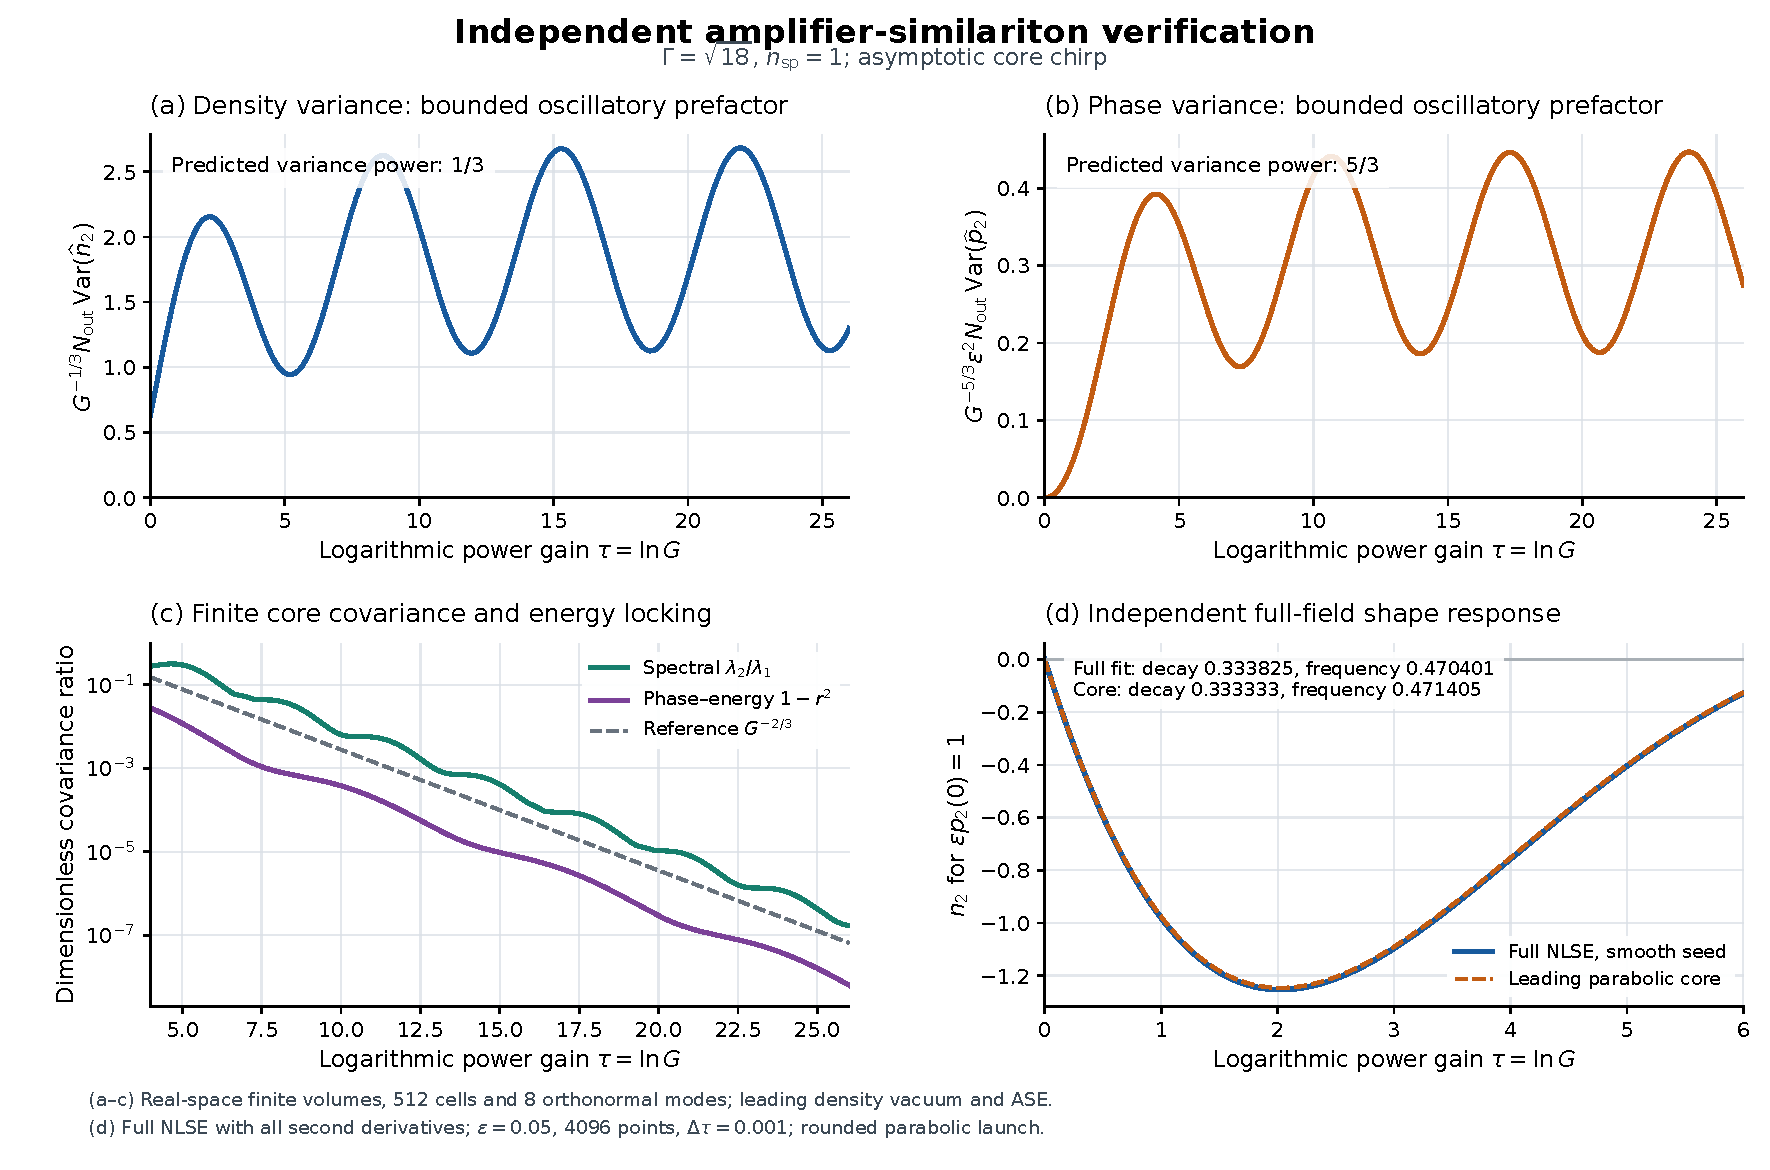
\includegraphics[width=\textwidth]{similariton_verification.pdf}
\caption{Independent similariton verification. Compensating the reduced variances by the predicted gain powers exposes bounded oscillatory envelopes. The spectral covariance and phase--energy deficit are finite-projection results. The full-field $l=2$ response independently checks the leading decay and oscillation. Corrected orthonormal finite-volume readouts are used.}
\end{figure}

\section{Problem 1 extensions: covariance, energy locking, and counterexamples}

\subsection{Which spectral covariance tends to rank one?}

For a strongly chirped mean, stationary phase maps time to frequency. Define $s(\xi_\omega)=\delta S(\omega)/S_{pk}$ on the spectral core, with $\xi_\omega=\omega/\omega_{edge}$. Linearizing the spectral density and its Jacobian gives
\begin{equation}\label{eq:specmap}
s_l=n_l-\frac{l(l+1)\eps_0}{aa_\zeta}p_l.
\end{equation}
On the asymptotic width this is $s_l=n_l+3n_{l,\tau}$. In particular, the repeated-root logarithm cancels for $l=1$, so $s_1=3b_1G^{-1/3}$. For $l\ge2$, $s_l$ is $G^{-1/3}$ times an oscillatory coefficient; $s_0=n_0$ retains an order-one energy variance.

The appropriate ordinary covariance is the covariance of \emph{orthonormal} coefficients
\begin{equation}
\widehat s_l=\sqrt{\frac{2}{2l+1}}s_l,\quad l=0,\ldots,4,
\qquad C_s=\Cov(\widehat s),\quad \mu_1\ge\mu_2\ge\cdots.
\end{equation}
Using the unweighted coefficient matrix instead changes its eigenvalues and numerical ratios. A common photon/energy factor does not change the ratio. The leading block structure is
\begin{equation}
C_s=\begin{pmatrix}
c_0+o(1)&G^{-1/3}b(\tau)^{\mathsf T}+o(G^{-1/3})\\
G^{-1/3}b(\tau)+o(G^{-1/3})&G^{-2/3}D(\tau)+o(G^{-2/3})
\end{pmatrix}.
\end{equation}
For $c_0>0$ and a conditional shape covariance $D-bb^{\mathsf T}/c_0$ whose largest eigenvalue is uniformly bounded above and away from zero, its Schur complement proves
\begin{equation}
\boxed{\mu_2/\mu_1=\Theta(G^{-2/3})}
\end{equation}
in this fixed finite-dimensional projection, with a generally oscillatory prefactor. This is an energy-dominated \emph{intensity-readout} covariance, not the covariance of all optical quadratures and not a rank-one pure quantum state.

\subsection{Matched-mean phase and the incorrect collective gain power}

The matched LO reads the normalized photon-number quadrature $X_A$ and the intensity-weighted phase $\bar p$:
\begin{equation}
n_0=\frac23\frac{\delta\Nph}{\Nph},\quad
X_A=\frac32\sqrt{\Nph}\,n_0,\qquad
\bar p=\frac34\int_{-1}^1(1-\xi^2)p\dd\xi=p_0-\frac15p_2,\quad
P_{LO}=2\sqrt{\Nph}\,\bar p.
\end{equation}
Number conservation of the Kerr/dispersion dynamics plus the gain reservoir gives the exact bright-field identity
\begin{equation}
C_{AA}=2n_{sp}G-(2n_{sp}-1).
\end{equation}
Let $\Phi_{NL}=\int_0^z\gamma P_{pk}(s)\dd s$. From \eqref{eq:asymwidth},
\begin{equation}
\Phi_{NL}\sim\frac{3}{2\Gamma\eps_0 A_G}G^{2/3}.
\end{equation}
Early energy noise dominates $p_0\simeq\Phi_{NL}n_0$, giving
\begin{equation}
\Var(p_0)\sim\frac{8n_{sp}}{9N_0}\Phi_{NL}^2,\qquad
\boxed{C_{PP}\sim\frac{32n_{sp}}9G\Phi_{NL}^2\propto\frac{G^{7/3}}{\eps_0^2}.}
\end{equation}
Thus the card's statement $C_{PP}\propto G/\eps_0^2$ omits the growing nonlinear-phase factor. This discrepancy is already visible in its own table of $\eps_0^2 C_{PP}/G$, which increases rapidly with gain. It is a genuine incorrect asymptotic statement, not a different quadrature convention.

For $r=\operatorname{Corr}(\bar p,\delta\Nph)$,
\begin{equation}
1-r^2=\frac{\Var(\bar p\mid\delta\Nph)}{\Var(\bar p)}.
\end{equation}
The leading shape residual is the $p_2$ component, whose unnormalized variance is $G^{2/3}$, whereas the energy-driven phase variance is $G^{4/3}$. Generically their ratio is therefore $\Theta(G^{-2/3})$. Late-injected energy noise supplies a smaller residual under these assumptions. Again, a constant limiting coefficient is not guaranteed in the presence of log-gain mode oscillations.

The independent reduced calculation reproduces the card's unchirped-seed values:
\begin{center}
\begin{tabular}{@{}lrr@{}}\toprule
$\tau=gL$ & $\mu_2/\mu_1$ & $1-r^2$ \\\midrule
4 & 0.3735559 & 0.01250545 \\
6 & 0.1095325 & 0.004355963 \\\bottomrule
\end{tabular}
\end{center}
These are 1024-cell values; for example, the card's source JSON gives 0.3735495 for the first spectral ratio. For the asymptotically chirped launch at $\tau=12,15,18$, the independent ratios are approximately $3.03109\times10^{-3},4.14125\times10^{-4},6.07135\times10^{-5}$, and the deficits $8.96326\times10^{-5},9.58672\times10^{-6},1.83660\times10^{-6}$. These reproduce the claimed values within the resolved spatial and quadrature error, without the repository implementation.

\subsection{Complete ASE does not rule out squeezing}

For a smooth coherent mean and its matched LO, differentiate the full covariance \eqref{eq:ase} at $z=0$. Passive dispersion has zero symmetric part at vacuum. Gain drift and ASE contribute $2n_{sp}gI$, while Kerr supplies an off-diagonal shear. The smallest matched-LO eigenvalue has right derivative
\begin{equation}\label{eq:counter}
\left.\frac{\dd\lambda_{LO}}{\dd z}\right|_{0^+}
=2n_{sp}g-2\gamma\frac{\int P^2\dd t}{\int P\dd t}.
\end{equation}
For the parabolic profile the ratio is $4P_0/5$, so the derivative is negative if $\gamma P_0>5n_{sp}g/4$. Smooth approximations to the parabola preserve this strict inequality. The literal sharp square-root parabola is outside the classical $H^2$ NLSE generator domain, so the rigorous derivative statement uses such smooth approximations. A smooth Gaussian gives the equally explicit condition $\gamma P_0>\sqrt2 n_{sp}g$. Therefore phase-insensitive amplifier noise does not prohibit a simultaneously nonlinear device from producing any squeezed quadrature.

The full lens-coordinate calculation, including both vacuum quadratures and both distributed ASE quadratures, supplies a numerical counterexample near a smoothed parabolic launch:
\begin{equation}
\eps_0=0.05,\quad \Gamma=\sqrt{18},\quad n_{sp}=1,\quad \tau=0.02,
\qquad
C_{LO}=\begin{pmatrix}
1.0404026801&0.1560393896\\
0.1560393896&1.0656702589
\end{pmatrix}.
\end{equation}
It has $\lambda_{LO}=0.8964864655$ (about $-0.475$ dB) and determinant $1.0843779023>1$. Grid/step refinement changes the minimum by $3.5\times10^{-9}$; the number-noise benchmark and reservoir-restored commutator agree to about $7\times10^{-14}$ in the refined short run.

This refutes the unconditional sentence ``with ASE there is no squeezing.'' It does not refute a more restricted assertion about late-gain matched-LO noise: the full-field $\tau=4,\eps_0=0.05$ case has $\lambda_{LO}\simeq3.159>1$. Indeed, in the reduced asymptotic model,
\begin{equation}
\lambda_{\min}(C_{LO})=\frac{\det C_{LO}}{\lambda_{\max}(C_{LO})}
\sim C_{AA}(1-r^2)=\Theta(G^{1/3}).
\end{equation}
Thus this specified matched mode eventually becomes noisier, under the same positive-envelope assumptions. This is the strongest minimally modified no-squeezing statement supported by the reduced calculation. It is not a theorem about every possible optical detection mode. The reported shape powers alone do not prove observable quantum squeezing, and ASE must be included in whichever covariance is optimized.

\subsection{Edges, gain bandwidth, initial data, and bright-field validity}

The full-field phase--energy deficit at $\tau=4$ is 0.02920071 for $\eps_0=0.05$ and 0.02841310 for $\eps_0=0.025$, approaching the leading asymptotic-launch value approximately 0.02804. The corresponding spectral ratios are about 0.31249 and 0.29547, versus a leading value about 0.278. The spectral readout is more sensitive to edge smoothing, Fourier resolution, and the stationary-phase approximation. The $\eps_0=0.025$ spectral ratio changes by about $8.8\times10^{-6}$ upon halving the fine distance step, although the collective deficit is much more stable. These numbers cannot be used to disprove a sharp-seed error bound, because the tested launch is deliberately smoothed; they also cannot prove that bound.

Four limits need to be kept separate:
\begin{enumerate}
\item \textbf{Hydrodynamic and edge limit.} Small bulk $\eps_{\mathrm{eff}}=\eps_0/\sqrt{Ga}$ does not uniformly control phase observables at a zero-density edge. A matched layer and its projection must be estimated. The claimed relative $O(\eps_0^2\log(1/\eps_0))$ covariance remainder remains unverified here.
\item \textbf{Large gain and bandwidth.} The chirped spectral edge grows approximately as $G^{1/3}$. With fixed gain bandwidth $\Omega_g$, a flatness condition such as $(\ln G)(\omega_{edge}/\Omega_g)^2\ll1$ eventually fails. The asymptotic laws are an intermediate regime or a joint bandwidth limit. Finite-bandwidth distortion of parabolic amplifiers has already been analyzed \cite{soh}.
\item \textbf{Initial-pulse dependence.} The exact separation uses a parabolic background. An unchirped parabola and an asymptotically chirped parabola have different transients and covariance prefactors. Arbitrary pulses can carry wings, chirp, and radiation; the attractor does not imply identical quantum covariance at finite gain. Known intermediate similariton dynamics already make this distinction \cite{wabnitz,kruglov}.
\item \textbf{Quantum linearization.} A fixed $N_0\ge10^4$ is not sufficient uniformly in gain. Since $\Var(p_0)\sim8n_{sp}\Phi_{NL}^2/(9N_0)$, a sufficient small-phase requirement is $\Phi_{NL}^2/N_0\ll1$. At $\eps_0=0.05,\Gamma=\sqrt{18},\tau=12$, $\Phi_{NL}\simeq2.11\times10^4$, so $N_0=10^4$ gives an rms uniform phase near 199 radians. At $\tau=18$, the same estimate requires $N_0$ much larger than $10^{12}$. A joint bright-field limit is needed for the very high-gain linearized phase asymptotic.
\end{enumerate}

\section{Problem 2: weak normal dispersion and the oscillator reduction}

\subsection{Exact anchor and the singular nature of the limit}

For a passive Gaussian pulse set $s=z/L$, $x=t/T_0$, $u=A/\sqrt{P_0}$,
\begin{equation}
\Phi=\gamma P_0L,\qquad \delta=\frac{\beta_2L}{T_0^2}=\frac L{L_D}>0,\qquad y=\Phi\delta,
\qquad u(0,x)=e^{-x^2/2}.
\end{equation}
The mean and its exact linearization are
\begin{align}\label{eq:weakmean}
u_s&=-\frac{i\delta}{2}u_{xx}+i\Phi|u|^2u,\\
v_s&=-\frac{i\delta}{2}v_{xx}+i\Phi(2|u|^2v+u^2v^*).
\end{align}
At $\delta=0$, $u=\sqrt p\,e^{i\Phi p s}$, where $p(x)=e^{-x^2}$. Removing the mean phase gives the local shear
\begin{equation}
M_0(x)=\begin{pmatrix}1&0\\2\Phi p(x)&1\end{pmatrix},\quad
v_-(q)=(\sqrt{1+q^2}-q)^2,\quad
\lzero=v_-(\Phi)=\frac1{(\sqrt{1+\Phi^2}+\Phi)^2}.
\end{equation}
The inverse-square expression avoids cancellation in numerical evaluation. Because $p$ has its unique maximum at one point, $\lzero$ is an \emph{unattained continuum infimum}, not an $L^2$ eigenvalue: any finite-width normalized mode samples smaller power away from the peak. A sequence of increasingly localized modes approaches it. Consequently analytic perturbation theory about a fixed isolated eigenvector at $\delta=0$ is not applicable. The optimizing mode itself changes width as dispersion is reduced.

\subsection{Derivation directly from the full generator}

Let the peak be $p(x)=1-\kappa x^2+O(x^4)$ with $\kappa>0$, and write $S=\sqrt{1+\Phi^2}$. Introduce the rescaling
\begin{equation}
\epsilon=\sqrt y,\qquad x=\sqrt\epsilon\,q,\qquad D=-\partial_q^2.
\end{equation}
After removing the evolving mean phase, the real fluctuation generator through first order is
\begin{equation}
G_\epsilon=G_0+\epsilon G_1+O(\epsilon^2),\quad
G_0=\begin{pmatrix}0&0\\2\Phi&0\end{pmatrix},\quad
G_1=\begin{pmatrix}
0&-D/(2\Phi)\\D/(2\Phi)-2\Phi\kappa q^2&0
\end{pmatrix}.
\end{equation}
The leading mean reshaping is order $y=\epsilon^2$; it cannot change the first coefficient. The Duhamel integral for propagation to $s=1$ is explicit:
\begin{equation}
M_1=\int_0^1e^{(1-s)G_0}G_1e^{sG_0}\dd s
=\begin{pmatrix}
-D/2&-D/(2\Phi)\\
(1/(2\Phi)-\Phi/3)D-2\Phi\kappa q^2&-D/2
\end{pmatrix}.
\end{equation}
Let $e_-$ be the normalized eigenvector of $M_0M_0^{\mathsf T}$ with eigenvalue $\lzero$. Projecting $V_1=M_1M_0^{\mathsf T}+M_0M_1^*$ gives
\begin{equation}\label{eq:effective}
\boxed{\lzero^{-1}e_-^{\mathsf T}V_1e_-
=\frac{\Phi}{S}\left(\frac D3+2\kappa q^2\right).}
\end{equation}
This full-generator derivation confirms the repository's continuous-wave balance while checking the matrix ordering and the evolving pulse background. In original $x$ coordinates the relative excess operator is
\begin{equation}\label{eq:osc}
H=-b\partial_x^2+\alpha x^2,\qquad
b=\frac{\delta\Phi^2}{3S},\qquad \alpha=\frac{2\Phi\kappa}{S}.
\end{equation}

\begin{proposition}[Exact effective-operator minimum]
For $b,\alpha>0$ and $\|f\|_2=1$,
\begin{equation}
b\|f'\|_2^2+\alpha\|xf\|_2^2\ge\sqrt{b\alpha},
\end{equation}
with equality at the normalized Gaussian $f(x)\propto\exp[-\sqrt{\alpha/b}\,x^2/2]$.
\end{proposition}
\begin{proof}
Integration by parts gives
$\|\sqrt b\,f'+\sqrt\alpha\,xf\|_2^2
=b\|f'\|_2^2+\alpha\|xf\|_2^2-\sqrt{b\alpha}$.
Nonnegativity proves the bound; the first-order equation for equality gives the Gaussian.
\end{proof}
Hence the leading optical branch has
\begin{equation}\label{eq:sqrtlaw}
\boxed{\frac{\lambda}{\lzero}-1
\sim\sqrt{\frac{2\kappa}{3}}\frac{\Phi}{\sqrt{1+\Phi^2}}\sqrt y,\qquad
\frac{\sigma_t}{T_0}\sim\left(\frac{y}{24\kappa}\right)^{1/4}.}
\end{equation}
Here $\sigma_t$ is the rms width of the normalized mode's squared amplitude, including both real quadrature components. For the Gaussian $\kappa=1$. The width coefficient holds at \emph{every fixed $\Phi>0$}, not only at large $\Phi$.

\subsection{Precisely where a global proof is still missing}

The oscillator proposition is rigorous. Taylor/Duhamel expansion on rescaled smooth localized test functions also constructs a quasimode of the full Bogoliubov covariance and the corresponding variational upper estimate. Turning this into equality for the \emph{global} continuum covariance infimum requires a matching lower bound excluding remote, rapidly oscillatory, or mixed-branch competing modes. This report has not completed that uniform microlocal estimate.

The exact frozen continuous-wave symbol supports the proposed localization. At local intensity $p$ and detuning $k$, let $a=\delta k^2/2$ and $\omega^2=a(a+2\Phi p)$. The smaller covariance eigenvalue is
\begin{equation}\label{eq:cwsymbol}
\lambda_{CW}=v_-\bigl(\Phi p\,|\sinc\omega|\bigr).
\end{equation}
For normal dispersion it has its unique global minimum at $p=1,a=0$, while large detuning returns toward vacuum. This removes an obvious sideband competitor at symbol level. However, a finite-time matrix propagator with rapidly oscillating dispersion symbols is not automatically covered by the scalar Schr\"odinger harmonic-approximation theorem. Simon's theorem \cite{simon} justifies the scalar mechanism, not the entire optical reduction without those additional estimates.

Thus the honest verdict is stronger than an unsupported scaling guess and narrower than a completed infinite-dimensional theorem: the coefficient is independently derived from the full equations, the exact reduced minimization is proved, and independent full-field spectra reproduce it; the global analytical identification of the lowest branch remains conditional on localization.

\subsection{Flat maxima: coefficient as well as exponent}

For $1-p(x)\sim\kappa x^{2m}$, $m\ge1$, the same projected kinetic term competes with $(2\Phi\kappa/S)x^{2m}$. Scaling to the anharmonic oscillator $-\dd^2/\dd q^2+q^{2m}$ with ground energy $e_{2m}$ gives
\begin{equation}\label{eq:flatlaw}
\boxed{\frac{\lambda}{\lzero}-1
\sim e_{2m}\left(\frac{2\kappa}{3^m}\right)^{1/(m+1)}
\frac{\Phi}{S}\,y^{m/(m+1)}.}
\end{equation}
The natural spatial scale is $(y/(6\kappa))^{1/(2m+2)}T_0$; rms width additionally contains the normalized ground-state rms. Independently diagonalizing the scalar oscillator and Richardson-extrapolating gives:
\begin{center}
\begin{tabular}{@{}rrrr@{}}\toprule
$2m$ & $e_{2m}$ & Excess coefficient before $(\Phi/S)y^{m/(m+1)}$ & Rms coefficient \\\midrule
2 & 1 & 0.81649658093 & 0.45180100180 \\
4 & 1.06036209028 & 0.64226859670 & 0.44635046932 \\
6 & 1.14480245368 & 0.59723755583 & 0.44355783696 \\\bottomrule
\end{tabular}
\end{center}
The last column multiplies $T_0y^{1/(2m+2)}$ for $\kappa=1$. A universal square root for ``any even, smooth pulse,'' as one open prediction in the card says, is false: $p=e^{-x^4}$ is already its own explicit counterexample. Multiple equal maxima would introduce several localized wells; an exactly flat plateau is a different limit again.

\subsection{A new second-order refinement}

For the Gaussian, expanding the full mean and tangent equations one order further yields the formal local branch expansion
\begin{equation}\label{eq:Bexp}
\frac{\lambda}{\lzero}-1=A(\Phi)\sqrt y+B(\Phi)y+O(y^{3/2}),\qquad
A(\Phi)=\sqrt{\frac23}\frac{\Phi}{S},
\end{equation}
with
\begin{equation}\label{eq:B}
\boxed{B(\Phi)=\frac{45+81\Phi^2+56\Phi^4+40\Phi^3S}{120\Phi S^3}.}
\end{equation}
Equivalently, writing the excess as $A\sqrt y[1+c_2\sqrt y+\cdots]$,
\begin{equation}\label{eq:c2}
\boxed{c_2(\Phi)=\frac{\sqrt6[45+81\Phi^2+56\Phi^4+40\Phi^3S]}{240\Phi^2(1+\Phi^2)},\qquad
c_2(\infty)=\frac{2\sqrt6}{5}=0.9797958971.}
\end{equation}
This refines the card's empirical $c_2\simeq1$; it does not contradict that approximate numerical observation.

To make the derivation reproducible rather than a fitted formula, the companion symbolic script expands, with $x=\sqrt\epsilon q$, the mean density and phase as
\begin{align}
\rho&=1-\epsilon q^2+\epsilon^2(q^4/2-s^2)+O(\epsilon^3),\\
\theta&=\Phi s-\epsilon\Phi s q^2
+\epsilon^2(\Phi s q^4/2-\Phi s^3/3+s/(2\Phi))+O(\epsilon^3).
\end{align}
The second generator has diagonal $-s(2q\partial_q+1)$, upper-right $1/(2\Phi)$, and lower-left $\Phi q^4-2\Phi s^2-1/(2\Phi)$. The time-ordered $G_1G_1$ term, the $G_2$ Duhamel term, the noncommutation of $D$ and $q^2$, and the mixing with the other quadrature branch all contribute. The branch-mixing correction is
\begin{equation}
-\frac{\|e_+^{\mathsf T}V_1(e_-f_0)\|_2^2}{\lzero^{-1}-\lzero}.
\end{equation}
This term contributes to the absolute eigenvalue's second-order coefficient; its sum with the $V_2$ expectation is divided by $\lzero$ to obtain the relative-excess coefficient $B$. Leaving out mean reshaping or using a commuting local symbol does not recover \eqref{eq:B}. The script derives the coefficient and checks the leading term symbolically; it does not insert the closed form as input.

Representative predicted values are $c_2(2)=1.01069098$, $c_2(3)=0.98946456$, $c_2(10)=0.98034160$, and $c_2(40)=0.97982793$. Refined full propagation at $\Phi=3,y=10^{-7}$ gives an effective coefficient 0.98943; at $\Phi=10,y=10^{-6}$ it gives 0.97998, consistent with the next $O(\sqrt y)$ correction and numerical cancellation. This is a formal local refinement with independent numerical support. A uniform global $O(y^{3/2})$ remainder has not been proved.

\section{Independent weak-dispersion computations and order of limits}

\subsection{Numerical method and convergence}

The main independent solver uses eighth-order centered periodic finite differences for $\partial_x^2$ and adaptive DOP853 integration in $s$. With $u=a+ib$, its exact real tangent equations are
\begin{align}
Q_s&=\frac\delta2D_2P_q-2\Phi abQ-\Phi(a^2+3b^2)P_q,\\
(P_q)_s&=-\frac\delta2D_2Q+\Phi(3a^2+b^2)Q+2\Phi abP_q.
\end{align}
For offsets $0,\pm1,\ldots,\pm4$, $D_2$ has coefficients $-205/72,8/5,-1/5,8/315,-1/560$, divided by $\Delta x^2$. Mean propagation is integrated independently with dense output; the tangent equation uses that trajectory. No split-step formulas from the repository are used.

To reduce cost, most runs launch a complete pair of canonical input columns only in a central support interval, while retaining all output rows. If $T=MP_{in}$, then $\|T\|\le\|M\|$, and $1/\|T\|^2$ is a variational \emph{upper bound} on the full minimum. Support enlargement and one complete tangent calculation verify that the relevant singular vector is contained. The $J$-rotated largest output singular vector gives the squeezed mode in the converged full-support limit. A truncated input calculation is not itself a complete covariance state.

The suite contains Gaussian cases at $\Phi=3,10$, quartic and sextic peaks at $\Phi=3$, $10^{-6}\le y\le10^{-2}$, and grid, support, window, zero-dispersion, and tolerance checks. The typical window is $|x|<4$; 1024 points are used, increased to 2048 or more for the narrowest Gaussian modes. All grids have uniform canonical quadrature normalization. For the smallest mode $\sigma_x\simeq0.0143$, grid spacing is substantially smaller than its rms width.

\begin{center}
\begin{tabular}{@{}rrrr@{}}\toprule
$\Phi$ & $y$ & Independent $\lambda_{\min}$ & Excess / leading formula \\\midrule
3 & $10^{-6}$ & 0.0263544574334 & 1.000990 \\
3 & $10^{-5}$ & 0.0263987454989 & 1.003125 \\
3 & $10^{-4}$ & 0.0265400309066 & 1.009850 \\
3 & $10^{-3}$ & 0.0269989825539 & 1.030841 \\
3 & $10^{-2}$ & 0.0285661909712 & 1.094286 \\
10 & $10^{-6}$ & 0.00248960058138\textsuperscript{a} & 1.000980 \\
10 & $10^{-4}$ & 0.00250798520186 & 1.009769 \\
10 & $10^{-2}$ & 0.00270875132945 & 1.094368 \\\bottomrule
\end{tabular}
\end{center}
\textsuperscript{a}Refined 3072-point, $2\times10^{-13}$ tolerance run, used because extracting a second coefficient from very small excesses amplifies integration error.

The fitted excess and width powers over $10^{-6}\le y\le10^{-4}$ are:
\begin{center}
\begin{tabular}{@{}lrrrr@{}}\toprule
Pulse and $\Phi$ & Excess power & Predicted & Width power & Predicted \\\midrule
Gaussian, 3 & 0.501914 & $1/2$ & 0.250240 & $1/4$ \\
Gaussian, 10 & 0.501899 & $1/2$ & 0.250148 & $1/4$ \\
$e^{-x^4}$, 3 & 0.667219 & $2/3$ & 0.166609 & $1/6$ \\
$e^{-x^6}$, 3 & 0.750317 & $3/4$ & 0.124926 & $1/8$ \\\bottomrule
\end{tabular}
\end{center}
At $\Phi=3,y=10^{-4}$ the measured rms width is 0.0452351, compared with 0.0451801. At $y=10^{-6}$ it is 0.0142888, compared with 0.0142872. Both coefficient and localization are reproduced.

The decisive crosscheck uses the separately implemented fourth-order Fourier symplectic tangent solver: for $\Phi=3,y=10^{-4}$ it gives 0.02654003090684555, versus 0.02654003090655749 with finite differences and DOP853, a relative difference about $1.1\times10^{-11}$. The two methods differ in spatial differentiation, propagation, tangent evaluation, and spectral optimization.

Convergence is not inferred solely from that agreement. Increasing 2048 to 3072 points at $\Phi=3,y=10^{-6}$ changes $\lambda$ by $4.0\times10^{-12}$ absolute. At $\Phi=3,y=10^{-3}$, same-grid support enlargement from 0.6 to 1.2 and then the entire input changes $\lambda$ by less than $6\times10^{-14}$; direct minimum versus reciprocal maximum agrees to $4.8\times10^{-14}$ relative in the full calculation. Increasing the half-window to 6 at fixed spacing also agrees. Tightening the tolerance at $\Phi=10,y=10^{-4}$ changes $\lambda$ by less than $4\times10^{-10}$ relative. Reported tangent symplectic and mean-energy errors are recorded for every case, usually about $10^{-11}$--$10^{-10}$ or smaller in the adaptive solver. The independent Fourier crosscheck has a bilinear symplectic defect $4.7\times10^{-15}$.

\begin{figure}[p]
\centering
\IfFileExists{../weak/weak_verification.pdf}{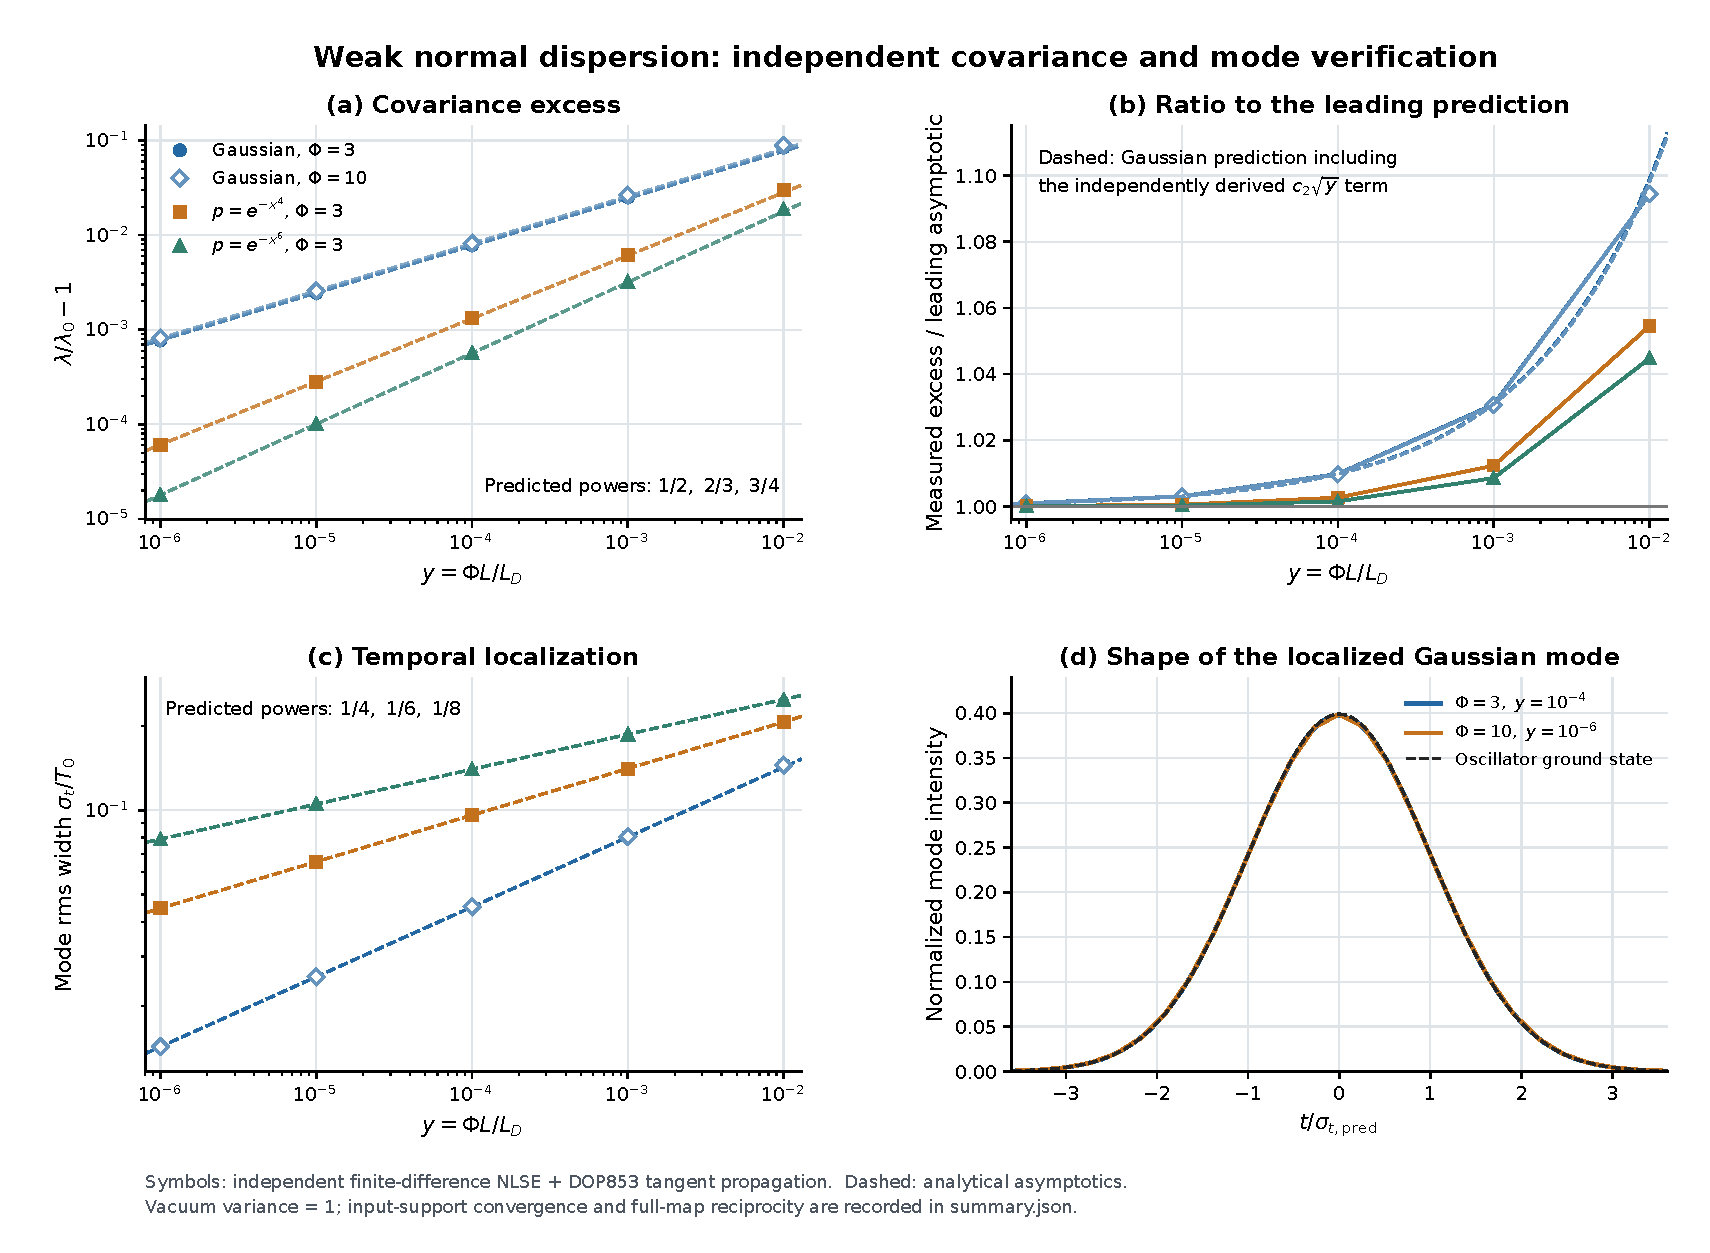
\includegraphics[width=\textwidth]{weak_verification.pdf}}{}
\caption{Independent full mean/tangent propagation for weak normal dispersion. The noninteger excess powers and shrinking detection-mode widths agree with the effective oscillator. Normalizing by the leading coefficient exposes the next correction. All points come from the verification code, not the repository's numerical output.}
\end{figure}

\subsection{Fixed $\Phi$, bandwidth, and a rigorous counterexample to a fixed-band interpretation}

The limit is $y\downarrow0$ at \emph{fixed $\Phi>0$}, after resolving the optimizing mode. It is not uniform in $\Phi\downarrow0$. The frozen dispersion symbol contains an $a^2$ term competing with $2a\Phi$; on the oscillator scale, a sufficient hierarchy in the joint small-$\Phi$ limit is $\sqrt y\ll\Phi^2$, or $\delta\ll\Phi^3$. The formulas at $\Phi=0$ must be replaced by the trivial vacuum covariance $I$.

The optimal temporal localization requires optical LO bandwidth $\Omega_bT_0\gg y^{-1/4}$ and grid spacing $\Delta t/T_0\ll y^{1/4}$. Optical envelope bandwidth is distinct from an RF detector's analysis window. At a fixed finite grid, eigenvalues are regular functions of dispersion near zero, and the Gaussian covariance minimum belongs to a different restricted problem.

There is a direct continuum fixed-band counterexample. Suppose a normalized vector LO is Fourier-limited to $|k|\le B=\Omega_bT_0$. Cauchy--Schwarz gives $|h(x)|^2\le B/\pi$. Choose $a_B=\pi/(4B)$; at least half its norm lies outside $[-a_B,a_B]$. Since the local smallest covariance eigenvalue increases away from the Gaussian maximum,
\begin{equation}\label{eq:bandbound}
\boxed{\lambda_{B,0}\ge\lzero+\frac12\left[v_-(\Phi e^{-a_B^2})-\lzero\right]>\lzero.}
\end{equation}
For large $B$, the relative lower gap is approximately $\pi^2\Phi/(16SB^2)$. Thus the quoted expansion about $\lzero$ cannot hold with the same vanishing excess at a fixed optical detection bandwidth. The unrestricted continuum limit is an essential part of the claim.

\subsection{Quantum ultraviolet and brightness restrictions}

At exactly zero dispersion with instantaneous response, the continuum Bogoliubov creation kernel is proportional to $p(x)\delta(x-x')$. It is not Hilbert--Schmidt on $L^2(\R)$, so the ideal transformation has infinite total spontaneous occupation and is not globally implementable as a finite-excitation vacuum Fock state without a bandwidth/material-response regulator. Individual smeared covariance measurements can still be meaningful. A finite temporal grid supplies a regulator, but its existence must not be mistaken for a physical material model. Finite response-time regularization was explicitly part of earlier broadband Kerr-noise theory \cite{joneckis}.

For $\delta>0$ the frozen-symbol estimate of the spontaneous occupation is finite and grows as $\delta^{-1/2}$ at fixed $\Phi$ as $\delta\downarrow0$. At large $\Phi$, its leading semiclassical estimate is
\begin{equation}
N_{ex}\ \text{of order}\ \frac{\Phi^2}{2\sqrt y}\int p^{3/2}(x)\dd x.
\end{equation}
For the Gaussian the integral is $\sqrt{2\pi/3}$. This is an estimate of the continuum trace from the frozen symbol, not a proved exact full-pulse trace asymptotic. It nevertheless explains why the card's $\Phi^2\ll\Nph$ is not a uniform brightness condition as the optimizing bandwidth diverges. Small depletion $N_{ex}\ll\Nph$ and adequate photons in the shrinking mode must be checked in any physical extrapolation. A finite material response, Raman noise, detector loss, or gain/loss must be included with its associated reservoir when present.

For completeness, the card's anomalous-dispersion wording also needs narrowing. In the frozen continuous-wave model, negative $a$ has the modulation-instability optimum at $a=-\Phi$, where $\lambda=e^{-2\Phi}$. Once that detuning is resolved, further grid bandwidth does not set the optimum. As $\beta_2\to0^-$ the optimum detuning diverges, so fixed-band and unrestricted limits do not commute. This is a counterexample to intrinsic perpetual cutoff dependence, not a certification of a pulsed anomalous-dispersion theorem.

\section{Strong normal dispersion: what the singular-value law proves}

\subsection{Scaling and hydrodynamic map}

For this claim $N$ is a nonlinear/dispersion parameter, \emph{not photon number}:
\begin{equation}
N^2=\frac{L_D}{L_{NL}},\quad \eps=N^{-1},\quad
Z=\frac z{\sqrt{L_DL_{NL}}},\quad \Phi=NZ,\quad y=Z^2.
\end{equation}
The scaled mean equation is $i\eps u_Z-\eps^2u_{xx}/2+|u|^2u=0$. At fixed $Z$, $N\to\infty$ implies $\Phi\to\infty$ but $z/L_D=Z/N\to0$: increasing power at fixed fiber length also changes $Z$ and is a different trajectory through parameter space.

Conjugating the field to use the conventional hydrodynamic signs, write phase $S/\eps$ and velocity $v=S_x$. Before gradient catastrophe,
\begin{equation}
\rho_Z+(\rho v)_x=0,\qquad S_Z+\frac12v^2+\rho=0.
\end{equation}
Their exact first variation for $\eta=\delta\rho,\psi=\delta S$ is
\begin{equation}
\eta_Z=-\partial_x(v\eta+\rho\psi_x),\qquad
\psi_Z=-v\psi_x-\eta.
\end{equation}
Using the common quadrature normalization (with the common field-to-photon unit factor understood), start with $\eta_0=\sqrt{\rho_0}X_0,\psi_0=0$ to define the amplitude-to-scaled-phase map
\begin{equation}
C_ZX_0=2\sqrt{\rho(Z)}\,\psi(Z).
\end{equation}
Conjugation changes its sign but not singular values. If physical phase quadrature is $Y=2\sqrt\rho\,\delta\phi$, the scaled coordinate is $\widetilde Y=\eps Y$. Rescaling both quadratures to Cartesian field variations would leave this same $C_Z$ map unchanged. Physical vacuum has covariance $I$ in $(X,Y)$ and $\operatorname{diag}(I,\eps^2I)$ in $(X,\widetilde Y)$. Assigning unit vacuum to both scaled coordinates would give the wrong squeezing problem.

\subsection{A proved finite-dimensional asymptotic}

\begin{lemma}\label{lem:strong}
Let a real symplectic physical-quadrature map have the form
\begin{equation}\label{eq:strongblock}
M_\eps=\begin{pmatrix}A_\eps&\eps B_\eps\\C_\eps/\eps&D_\eps\end{pmatrix}.
\end{equation}
Suppose $A_\eps=A_0+O(\eps^2)$, $C_\eps=C_0+O(\eps^2)$, $D_\eps=D_0+O(\eps^2)$, and $B_\eps=O(1)$ in a fixed finite-dimensional matrix norm, with $s_1=\sigma_1(C_0)>0$. Then
\begin{equation}\label{eq:stronglaw}
\boxed{\lambda_{\min}(M_\eps M_\eps^{\mathsf T})
=\frac{\eps^2}{s_1^2}[1+O(\eps^2)].}
\end{equation}
No inverse of $C_0$ is needed.
\end{lemma}
\begin{proof}
Put $K_\eps=\eps M_\eps$. Then
\begin{equation}
K_\eps K_\eps^{\mathsf T}=\begin{pmatrix}
\eps^2 A_0A_0^{\mathsf T}+O(\eps^4)&\eps A_0C_0^{\mathsf T}+O(\eps^3)\\
\eps C_0A_0^{\mathsf T}+O(\eps^3)&C_0C_0^{\mathsf T}+O(\eps^2)
\end{pmatrix}.
\end{equation}
The nonzero unperturbed eigenspaces are in the lower block. The order-$\eps$ perturbation has zero compression to them. A Schur complement for eigenvalues bounded away from zero therefore gives $\|K_\eps\|^2=s_1^2+O(\eps^2)$. Equation \eqref{eq:recip} completes the proof.
\end{proof}
For fixed blocks and a simple top singular vector $w$ of $C_0C_0^{\mathsf T}$, the next relative term is $-\eps^2 b/s_1^2$ with
\begin{equation}
b=\|D_0^{\mathsf T}w\|^2+\frac{\|A_0C_0^{\mathsf T}w\|^2}{s_1^2}.
\end{equation}
A physical $C_\eps=C_0+\eps^2C_2+\cdots$ adds $2w^{\mathsf T}C_2C_0^{\mathsf T}w$, which has no fixed sign. Thus the negative relative correction and the proposed bound $0<c(Z)\le2$ do not follow from symplecticity alone. The leading law can survive even if those extra coefficient assertions fail.

\subsection{Why continuum and wave-breaking qualifications are substantive}

Even before breaking, the bounded-block lemma does not immediately cover white continuum vacuum. On a constant background,
\begin{equation}
B_0(k)=-\frac{k}{2\sqrt\rho}\sin(k\sqrt\rho Z),\qquad
C_0(k)=\frac{2\sqrt\rho}{k}\sin(k\sqrt\rho Z).
\end{equation}
The first is unbounded on $L^2$. A finite smooth subspace or an appropriate Sobolev/microlocal estimate is required, together with convergence of the relevant extremal spectrum.

At gradient catastrophe the smooth Euler gradients diverge and the dispersive quantum-pressure term is no longer uniformly negligible. Known defocusing semiclassical analysis distinguishes smooth hydrodynamics from the oscillatory regime after breaking \cite{jin}. Its global results have their own initial-data hypotheses; they are not a theorem for the present Gaussian quantum covariance. Differentiating a weak limit of mean fields also need not commute with the semiclassical limit.

A meaningful amended postbreaking statement uses the \emph{full NLSE} tangent map
\begin{equation}
M_N=\begin{pmatrix}A_N&B_N/N\\NC_N&D_N\end{pmatrix}.
\end{equation}
If $C_N\to C_\infty$ in operator norm, $\|A_N\|/N\to0$, $\|D_N\|/N\to0$, and $\|B_N\|/N^2\to0$, then $M_N/N$ tends to the lower-left block and symplectic reciprocity proves
\begin{equation}
N^2\lambda_{\min}(V_N)\longrightarrow\|C_\infty\|^{-2}.
\end{equation}
This implication is rigorous. Establishing the hypotheses across dispersive shocks is a separate problem. The present computations support a principal squeezing limit at the tested postbreaking distance, not all of those operator-norm conditions.

\subsection{Independent full-field and hydrodynamic results}

The full-field implementation uses a fourth-order Yoshida composition of exact Fourier dispersion and exact Kerr subflows, together with their exact tangent and real adjoint maps. It keeps the complete quadrature grid, with no attenuation or anti-alias window that would silently remove quantum noise. A matrix-free extremal eigensolver uses \eqref{eq:recip}; selected small cases are also verified by dense direct covariance diagonalization. The independent hydrodynamic solver evolves the dispersionless mean and exact tangent on a complete grid using DOP853, without the repository's Hermite input basis.

\begin{center}
\begin{tabular}{@{}rrrrr@{}}\toprule
$Z$ & $N$ & $\lambda_{\min}$ & $N^2\lambda_{\min}$ & $N^2\lambda_2$ \\\midrule
0.75 & 10 & 0.00849475491909 & 0.849475491909 & 2.10329262171 \\
0.75 & 20 & 0.00214861598479 & 0.859446393918 & 2.16001418543 \\
0.75 & 40 & 0.000538743360285 & 0.861989376456 & 2.17499614549 \\
1.50 & 10 & 0.00360415762994 & 0.360415762994 & 1.38497212453 \\
1.50 & 20 & 0.000904781621298 & 0.361912648519 & 1.41958221733 \\
1.50 & 40 & 0.000226416782641 & 0.362266852226 & 1.43027064468 \\\bottomrule
\end{tabular}
\end{center}
Before breaking, the independent hydrodynamic coefficients are
\begin{equation}
\Lambda(0.75)=0.86284166134396,\qquad \Pi(0.75)=2.18007053159266.
\end{equation}
The relative leading-law deficits at $N=10,20,40$ are $1.5491\%,0.3935\%,0.0988\%$, with fitted error power $-1.98555$. This reproduces both the leading coefficient and the expected prebreaking $N^{-2}$ relative correction. At $Z=1.5$, the full-field values approach the repository's approximately 0.3625 coefficient and support the leading $N^{-2}$ law at this tested postbreaking point. They do not establish a universal next-error exponent there.

For $N=20,Z=1.5$, changing $(\text{points},\text{window},\text{steps})$ from $(512,16,600)$ to $(1024,16,1200)$ and $(1024,32,1200)$ gives respectively
\begin{equation}
0.0009047816213077796,\quad
0.0009047816212975458,\quad
0.0009047816212980431.
\end{equation}
The minimum is stable to about $1.2\times10^{-11}$ relative under these changes. Dense symplectic defects are about $2\times10^{-13}$; direct/reciprocal minima agree to several $10^{-12}$ relative. The number-conservation gradient identity is checked as well. The amplitude block grows after breaking (approximately 1.66, 2.22, 3.34 for the three $N$ values), and $\sigma_1(C_N)^{-2}$ is more cutoff-sensitive than $\lambda_{\min}$: it changes by about $1.6\times10^{-5}$ relative in a grid refinement at $N=20$. Convergence of the covariance minimum alone is not convergence of every hydrodynamic block.

\begin{figure}[p]
\centering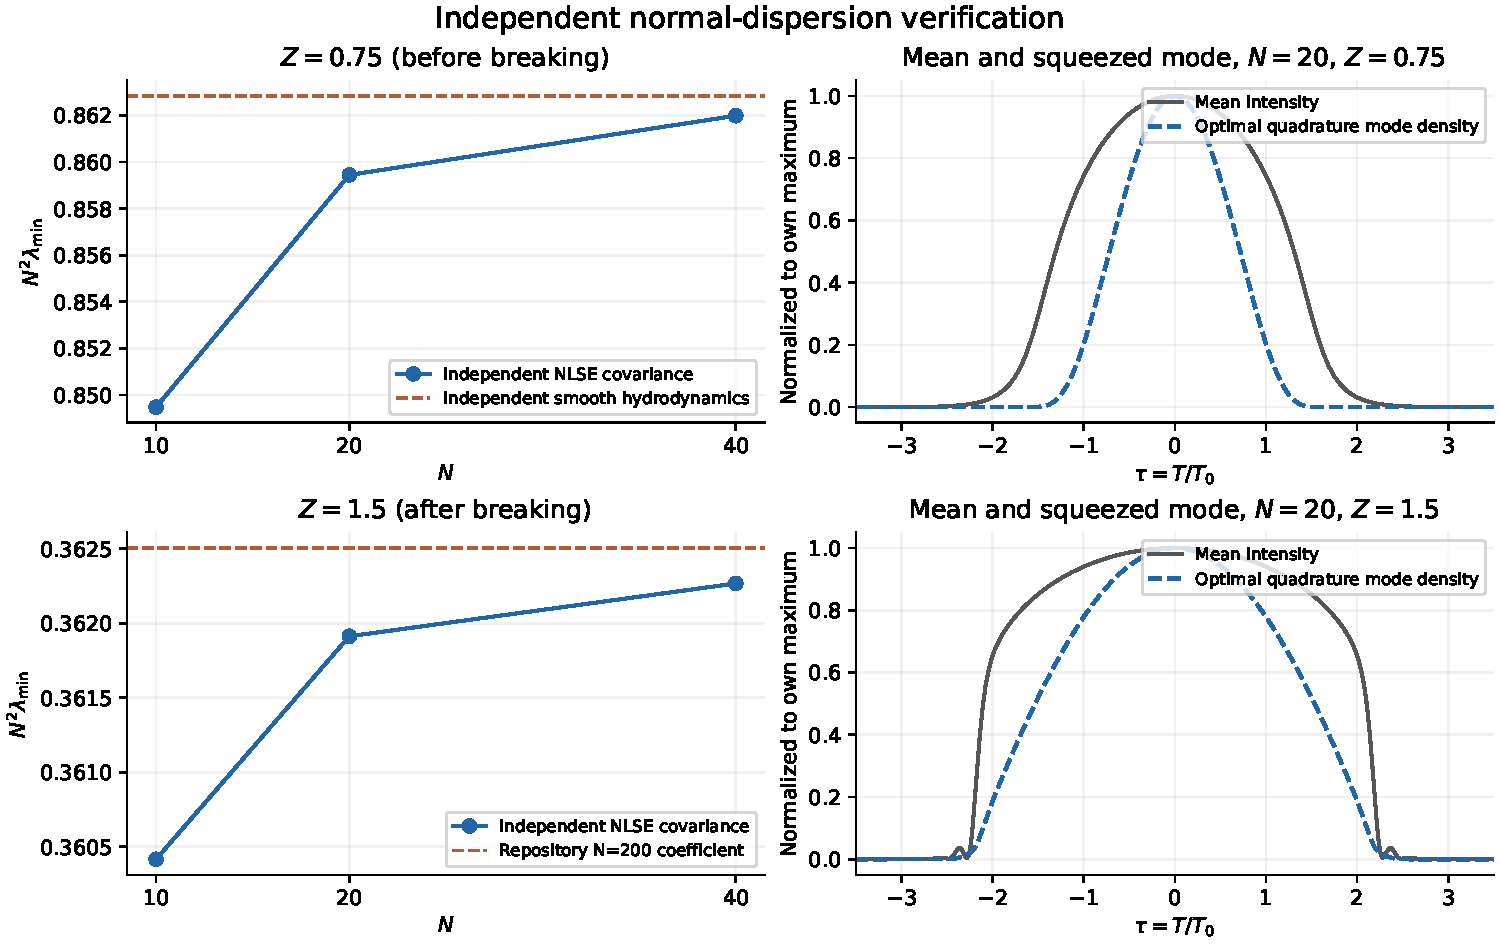
\includegraphics[width=\textwidth]{strong_comparison.pdf}
\caption{Independent strong-dispersion calculations. The prebreaking coefficient comes from a separate zero-dispersion hydrodynamic tangent calculation; the postbreaking points come from the full NLSE. The figure distinguishes a reproduced finite-$N$ trend from a theorem identifying the postbreaking limit.}
\end{figure}

\subsection{Detection modes, small-$Z$ overlap, and basis bias}

The first three squeezed eigenvectors in the full calculation have parity even, odd, even. An exact passive-readout hyperplane projection gives $\lambda_{pass}=\lambda_2$ in the dense tested cases. Parity alone only guarantees an admissible odd candidate; it does not prove that all admissible even modes lie higher. The exactly odd mode is dark relative to an even coherent pulse, so bright-field photon counting approaches its quadrature variance by a small even carrier admixture with sufficient detected photons, or the quadrature can be measured by an external LO. An exactly dark output cannot be assigned the same bright-field Fano normalization. The optimum physical modes also contain the rapidly varying output mean phase; optical detection must resolve that chirp as $N$ increases. A fixed spectral filter or fixed LO is an additional constraint on the asymptotic readout.

The small-$Z$ hydrodynamic singular-mode oscillator gives
\begin{equation}
4Z^2\Lambda(Z)=1+\sqrt{2/3}\,Z+O(Z^2),\qquad
4Z^2\Pi(Z)=1+\sqrt6\,Z+O(Z^2).
\end{equation}
Because $y=Z^2$ and $\Phi\to\infty$ in this overlap, the first coefficient is the same result as the weak-dispersion square root. It should not be counted as a separate discovery.

A useful numerical refinement is isolated at $Z=0.1$. Complete-grid hydrodynamics gives $\Lambda=27.2339599259846$, $\Pi=31.9800336840980$. Projecting that same independently calculated map onto 80 Hermite input functions gives $\Lambda_{H80}=27.2372686197941$, $\Pi_{H80}=32.0326726605127$, reproducing the repository's \path{hydro_direct.json}. The Hermite Gram defect is $4.1\times10^{-15}$, so the difference is basis truncation, not normalization. The biases are about $0.012\%$ and $0.165\%$. This changes a precision assessment, not the leading scaling law.

\section{Correctness versus novelty: comparison with primary literature}

The literature search was directed at the mathematical mechanism and the closest physical antecedents, including the papers cited by the repository. Relevant primary text was read where accessible; abstract-only access is stated below. This is a bounded priority search, not proof that no earlier expression exists.

\begin{longtable}{@{}p{.26\textwidth}p{.44\textwidth}p{.24\textwidth}@{}}
\toprule
Primary source & Relevance to the present claims & Access used \\\midrule\endhead
Fermann et al. (2000); Kruglov et al. (2002) \cite{fermann,kruglov} & Parabolic amplifier similariton, self-similar gain/width scaling, attraction and low-amplitude wings. These ingredients are established. & Fermann full paper; Kruglov publisher abstract and primary-paper text inspected by a parallel verifier. \\
Wabnitz (2007) \cite{wabnitz} & Classical parabolic-parameter dynamics and spiral approach to the similariton. Linearizing the width equation already gives the $l=2$ decay mechanism used here. & Full author-uploaded two-page conference paper; journal abstract. \\
Menotti--Stringari (2002); Fedichev--Fischer (2004) \cite{menotti,fedichev} & The parabolic hydrodynamic mode spectrum and expanding-background mode separation have close condensate antecedents. & Full primary preprints, relevant equations. \\
Caves (1982); Drummond--Corney (2000/2001) \cite{caves,drummondcorney} & Quantum amplifier noise, commutator preservation, and fiber reservoir equations. & Primary abstract and author PDF for Caves; full preprint for fiber stochastic equations. \\
Soh--Nilsson--Grudinin (2006) \cite{soh} & Finite gain bandwidth distorts chirp and spectral shape in parabolic amplification. & Publisher abstract. \\
Potasek--Yurke (1987); Drummond--Carter (1987) \cite{potasek,drummondcarter} & Dispersive Kerr squeezing and normal-dispersion spectral behavior precede these claims. & Primary publisher abstracts. \\
Joneckis--Shapiro (1993); Doerr--Shirasaki--Khatri (1994) \cite{joneckis,doerr} & Broadband quantum noise with finite response time, and linearized pulsed GVD squeezing. & Primary publisher abstracts; full older texts not obtained here. \\
Opatrn\'y--Korolkova--Leuchs (2002) \cite{opatrny} & Full covariance optimization, optimum LO, and lower bounds on filtering, including vacuum from partial transmission. & Full paper, especially Sections IV--VI, Eqs.\ (52)--(64). \\
Simon (1983) \cite{simon} & Harmonic-well semiclassical eigenvalue asymptotics are an established mathematical mechanism. & Full primary paper; optical matrix extension not assumed. \\
Braunstein (2005) \cite{braunstein} & Symplectic/SVD decomposition of Gaussian squeezing is established. & Full author PDF, theorem and appendix. \\
Jin--Levermore--McLaughlin (1999) \cite{jin} & Smooth defocusing hydrodynamics versus postbreaking oscillatory semiclassical limits. & Full primary author PDF, relevant prebreaking and breaking discussion. \\
Krylov--Bergman--Lai (1999) \cite{krylov} & Experimental squeezing in normal-dispersion fiber already existed. & Primary publisher abstract. \\
\bottomrule
\end{longtable}

\paragraph{Similariton novelty.} The background attractor, classical width relaxation, reservoir physics, and parabolic hydrodynamic eigenfunctions are prior art. The $g/3$ breathing rate follows by linearizing the already known width equation, so a broad first-ever analytical attraction-rate claim is unsafe. The particular extension to all fixed low-order shape modes, its quantum-normalized variance powers, and the specified spectral/phase covariance projections may be useful incremental results. No exact antecedent for the four requested projected-noise scalings was located in the primary sources inspected, but this remains provisional. A 2016 SPIE paper explicitly titled intensity-noise reduction in a self-similar parabolic amplifier is an additional close lead \cite{wang}; its full primary text was not obtained, so it is not used to assert either identical exponents or priority defeat.

\paragraph{Weak-dispersion novelty.} The strongest candidate is the \emph{specific} nonanalytic correction, its explicit coefficient for a Gaussian, the optimum-mode localization scale, and the peak-order generalization. Covariance eigenmode optimization, Kerr squeezing, normal-dispersion propagation, filtering bounds, and the oscillator mechanism are established separately. The search did not locate the displayed coefficient or its generalization in prior primary literature. Older full-text access gaps prevent an unqualified novelty claim. The new local $c_2(\Phi)$ formula in this verification is an additional refinement; its mathematical/global scope must be stated alongside it.

\paragraph{Strong-dispersion novelty.} The optimized function $\Lambda(Z)$ as a particular optical application is a plausible candidate contribution. Symplectic singular-value reasoning and the semiclassical hydrodynamic machinery are established. The overlap coefficient duplicates the weak result. A correct postbreaking tangent-spectrum theorem would be more ambitious and is not supplied by either the card's checks or this finite set of reproductions.

\section{Reproduction guide, provenance, and remaining verification gaps}

The companion archive contains all newly written solvers, raw JSON outputs, selected mode arrays, convergence records, detailed derivation notes, plotting scripts, and this LaTeX source. It excludes repository code and temporary dependency installations. The archive's repository inventory records the inspected snapshot paths and SHA-256 hashes; it lets an authorized reader compare source material against the pinned commit without redistributing the repository.

The primary independent paths are:
\begin{itemize}
\item \path{weak/verify_weak.py}, \path{weak/run_suite.py}: finite-difference mean/tangent solver and parameter/convergence sweep.
\item \path{weak_theory/second_order_symbolic.py}, \path{weak_theory/effective_oscillator.py}: symbolic second correction and independent oscillator constants.
\item \path{similariton/fv_covariance.py}, \path{similariton/lens_nlse.py}: finite-volume covariance and full lens-coordinate propagation with complete ASE.
\item The \path{strong} directory contains \path{verify_strong.py}, \path{verify_hydro.py}, and \path{verify_weak_cross.py}: symplectic Fourier propagation, direct hydrodynamics, and the cross-method weak test.
\item Each directory's README explains the precise commands and which outputs are asymptotic, variational bounds, or full finite-grid quantum covariances.
\end{itemize}

A normal Python environment with NumPy, SciPy, Matplotlib and SymPy reproduces the work. The recorded runtime used Python 3.12, NumPy 2.3.5 and SciPy 1.17.0; exact versions and numerical settings are in the archive. Running every parameter and high-resolution amplifier case may take appreciably longer than the quick checks. A fast entry point is the weak Fourier crosscheck, followed by the scalar oscillator and reduced covariance suite. No network access or repository imports are needed for these calculations.

\paragraph{Established within explicit models.} The leading similariton mode spectrum and variance-envelope algebra; finite-projection covariance Schur-complement law; matched collective phase $G^{7/3}$ correction; complete-noise short-length squeezing criterion; effective oscillator minimum and general peak scaling; fixed-band gap; and finite-dimensional symplectic $N^{-2}$ lemma.

\paragraph{Reliable numerical evidence.} Independent weak covariance minima and mode localization across Gaussian/quartic/sextic peaks; two full solvers agreeing at $10^{-11}$ relative on a common case; full-field low-order similariton behavior and complete ASE counterexample; independent prebreaking $\Lambda$ and a converged postbreaking $N$ sequence; identified Hermite truncation bias. Raw diagnostics substantiate these claims.

\paragraph{Unverified assumptions or extensions.} Uniform sharp-edge error estimates and all-mode amplifier covariance limits; physically accessible infinite-gain/fixed-brightness extrapolations; a matching global weak-dispersion lower bound; a uniform second-order remainder; continuum high-frequency control of the strong hydrodynamic blocks; and a postbreaking full-tangent operator limit. These are the concrete remaining gaps between the surviving leading results and stronger theorem-level claims.

\paragraph{Minimally modified claims recommended for the repository.} State the amplifier exponents as fixed-low-mode photon-normalized variance envelopes within the parabolic hydrodynamic interior, with complete-noise observability assessed separately. State the weak result as an independently supported singular asymptotic for unrestricted homodyne covariance at fixed $\Phi>0$, with the stated bandwidth/brightness limit and a conditional continuum proof. State strong squeezing as a symplectic finite-block theorem before breaking plus full-NLSE numerical evidence and an explicit tangent-limit conjecture after breaking. These changes preserve the strongest results while removing the unsupported conclusions.

\begin{thebibliography}{99}
\small
\bibitem{fermann} M. E. Fermann, V. I. Kruglov, B. C. Thomsen, J. M. Dudley and J. D. Harvey, ``Self-Similar Propagation and Amplification of Parabolic Pulses in Optical Fibers,'' \emph{Phys. Rev. Lett.} \textbf{84}, 6010--6013 (2000). \doi{10.1103/PhysRevLett.84.6010}. \href{https://discovery.ucl.ac.uk/97897/1/97897.pdf}{Primary paper PDF}.
\bibitem{kruglov} V. I. Kruglov, A. C. Peacock, J. D. Harvey and J. M. Dudley, ``Self-similar propagation of parabolic pulses in normal-dispersion fiber amplifiers,'' \emph{J. Opt. Soc. Am. B} \textbf{19}, 461--469 (2002). \doi{10.1364/JOSAB.19.000461}.
\bibitem{wabnitz} S. Wabnitz, ``Analytical dynamics of parabolic pulses in nonlinear optical fiber amplifiers,'' \emph{IEEE Photon. Technol. Lett.} \textbf{19}, 507--509 (2007), \doi{10.1109/LPT.2007.893823}; and ``Analytical Dynamics of Optical Similaritons,'' QELS/CLEO 2007, paper JWA71, \doi{10.1109/QELS.2007.4431461}. \href{https://www.researchgate.net/publication/238087766_Analytical_Dynamics_of_Optical_Similaritons}{Full primary conference paper uploaded by its author}.
\bibitem{menotti} C. Menotti and S. Stringari, ``Collective oscillations of a 1D trapped Bose gas,'' \emph{Phys. Rev. A} \textbf{66}, 043610 (2002). \href{https://arxiv.org/abs/cond-mat/0201158}{arXiv:cond-mat/0201158}.
\bibitem{fedichev} P. O. Fedichev and U. R. Fischer, ``Cosmological quasiparticle production in harmonically trapped superfluid gases,'' primary preprint, version of 10 March 2004. \href{https://arxiv.org/abs/cond-mat/0303063}{arXiv:cond-mat/0303063}.
\bibitem{caves} C. M. Caves, ``Quantum limits on noise in linear amplifiers,'' \emph{Phys. Rev. D} \textbf{26}, 1817--1839 (1982). \doi{10.1103/PhysRevD.26.1817}.
\bibitem{drummondcorney} P. D. Drummond and J. F. Corney, ``Quantum noise in optical fibers I: stochastic equations,'' primary preprint, 28 August 2000 version. \href{https://arxiv.org/abs/quant-ph/9912095}{arXiv:quant-ph/9912095}.
\bibitem{soh} D. B. S. Soh, J. Nilsson and A. B. Grudinin, ``Efficient femtosecond pulse generation using a parabolic amplifier combined with a pulse compressor. II. Finite gain-bandwidth effect,'' \emph{J. Opt. Soc. Am. B} \textbf{23}, 10--19 (2006). \doi{10.1364/JOSAB.23.000010}.
\bibitem{potasek} M. J. Potasek and B. Yurke, ``Squeezed-light generation in a medium governed by the nonlinear Schr\"odinger equation,'' \emph{Phys. Rev. A} \textbf{35}, 3974 (1987). \doi{10.1103/PhysRevA.35.3974}.
\bibitem{drummondcarter} P. D. Drummond and S. J. Carter, ``Quantum-field theory of squeezing in solitons,'' \emph{J. Opt. Soc. Am. B} \textbf{4}, 1565 (1987). \doi{10.1364/JOSAB.4.001565}.
\bibitem{joneckis} L. G. Joneckis and J. H. Shapiro, ``Quantum propagation in a Kerr medium: lossless, dispersionless fiber,'' \emph{J. Opt. Soc. Am. B} \textbf{10}, 1102--1120 (1993), with subsequent erratum. \doi{10.1364/JOSAB.10.001102}.
\bibitem{doerr} C. R. Doerr, M. Shirasaki and F. I. Khatri, ``Simulation of pulsed squeezing in optical fiber with chromatic dispersion,'' \emph{J. Opt. Soc. Am. B} \textbf{11}, 143--149 (1994). \doi{10.1364/JOSAB.11.000143}.
\bibitem{opatrny} T. Opatrn\'y, N. Korolkova and G. Leuchs, ``Mode structure and photon number correlations in squeezed quantum pulses,'' \emph{Phys. Rev. A} \textbf{66}, 053813 (2002). \doi{10.1103/PhysRevA.66.053813}. \href{https://arxiv.org/abs/quant-ph/0204131}{arXiv:quant-ph/0204131}.
\bibitem{simon} B. Simon, ``Semiclassical analysis of low lying eigenvalues. I. Non-degenerate minima: asymptotic expansions,'' \emph{Ann. Inst. H. Poincar\'e A} \textbf{38}, 295--308 (1983). \href{https://www.numdam.org/item/AIHPA_1983__38_3_295_0.pdf}{Primary paper PDF}.
\bibitem{braunstein} S. L. Braunstein, ``Squeezing as an irreducible resource,'' \emph{Phys. Rev. A} \textbf{71}, 055801 (2005). \doi{10.1103/PhysRevA.71.055801}. \href{https://www-users.york.ac.uk/~sb54/papers/b05B.pdf}{Author PDF}.
\bibitem{jin} S. Jin, C. D. Levermore and D. W. McLaughlin, ``The semiclassical limit of the defocusing NLS hierarchy,'' \emph{Commun. Pure Appl. Math.} \textbf{52}, 613--654 (1999). \href{https://math.nyu.edu/~dmac/docs/DWM-31.pdf}{Primary author PDF}.
\bibitem{krylov} D. Krylov, K. Bergman and Y. Lai, ``Photon-number squeezing in the normal-dispersion regime,'' \emph{Opt. Lett.} \textbf{24}, 774--776 (1999). \doi{10.1364/OL.24.000774}.
\bibitem{wang} S. Wang, B. Liu, Y. Song and M. Hu, ``Intensity noise reduction of a high-power nonlinear femtosecond fiber amplifier based on spectral-breathing self-similar parabolic pulse evolution,'' \emph{Proc. SPIE} \textbf{9893}, 98930J (2016). \doi{10.1117/12.2227743}. Full text not accessed; a priority-search lead only.
\end{thebibliography}
\end{document}
